\chapter{Obrazové přílohy}

\begin{figure}[htbp]
    \centering
    \includegraphics[width=0.85\textwidth]{img/prijimac-1.JPG}
    \caption{Fotografie přijímače Janus omni-ultra na robotovi zblízka.}
    \label{fig:prijimac1}
\end{figure}

\begin{figure}[htbp]
    \centering
    \includegraphics[width=0.85\textwidth]{img/prijimac-2.JPG}
    \caption{Fotografie přijímače Janus omni-ultra na robotovi ukazující svazek vodičů potřebných pro obsluhu senzorů HC-SR04 bez dodatečného procesoru.}
    \label{fig:prijimac2}
\end{figure}

\begin{figure}[htbp]
    \centering
    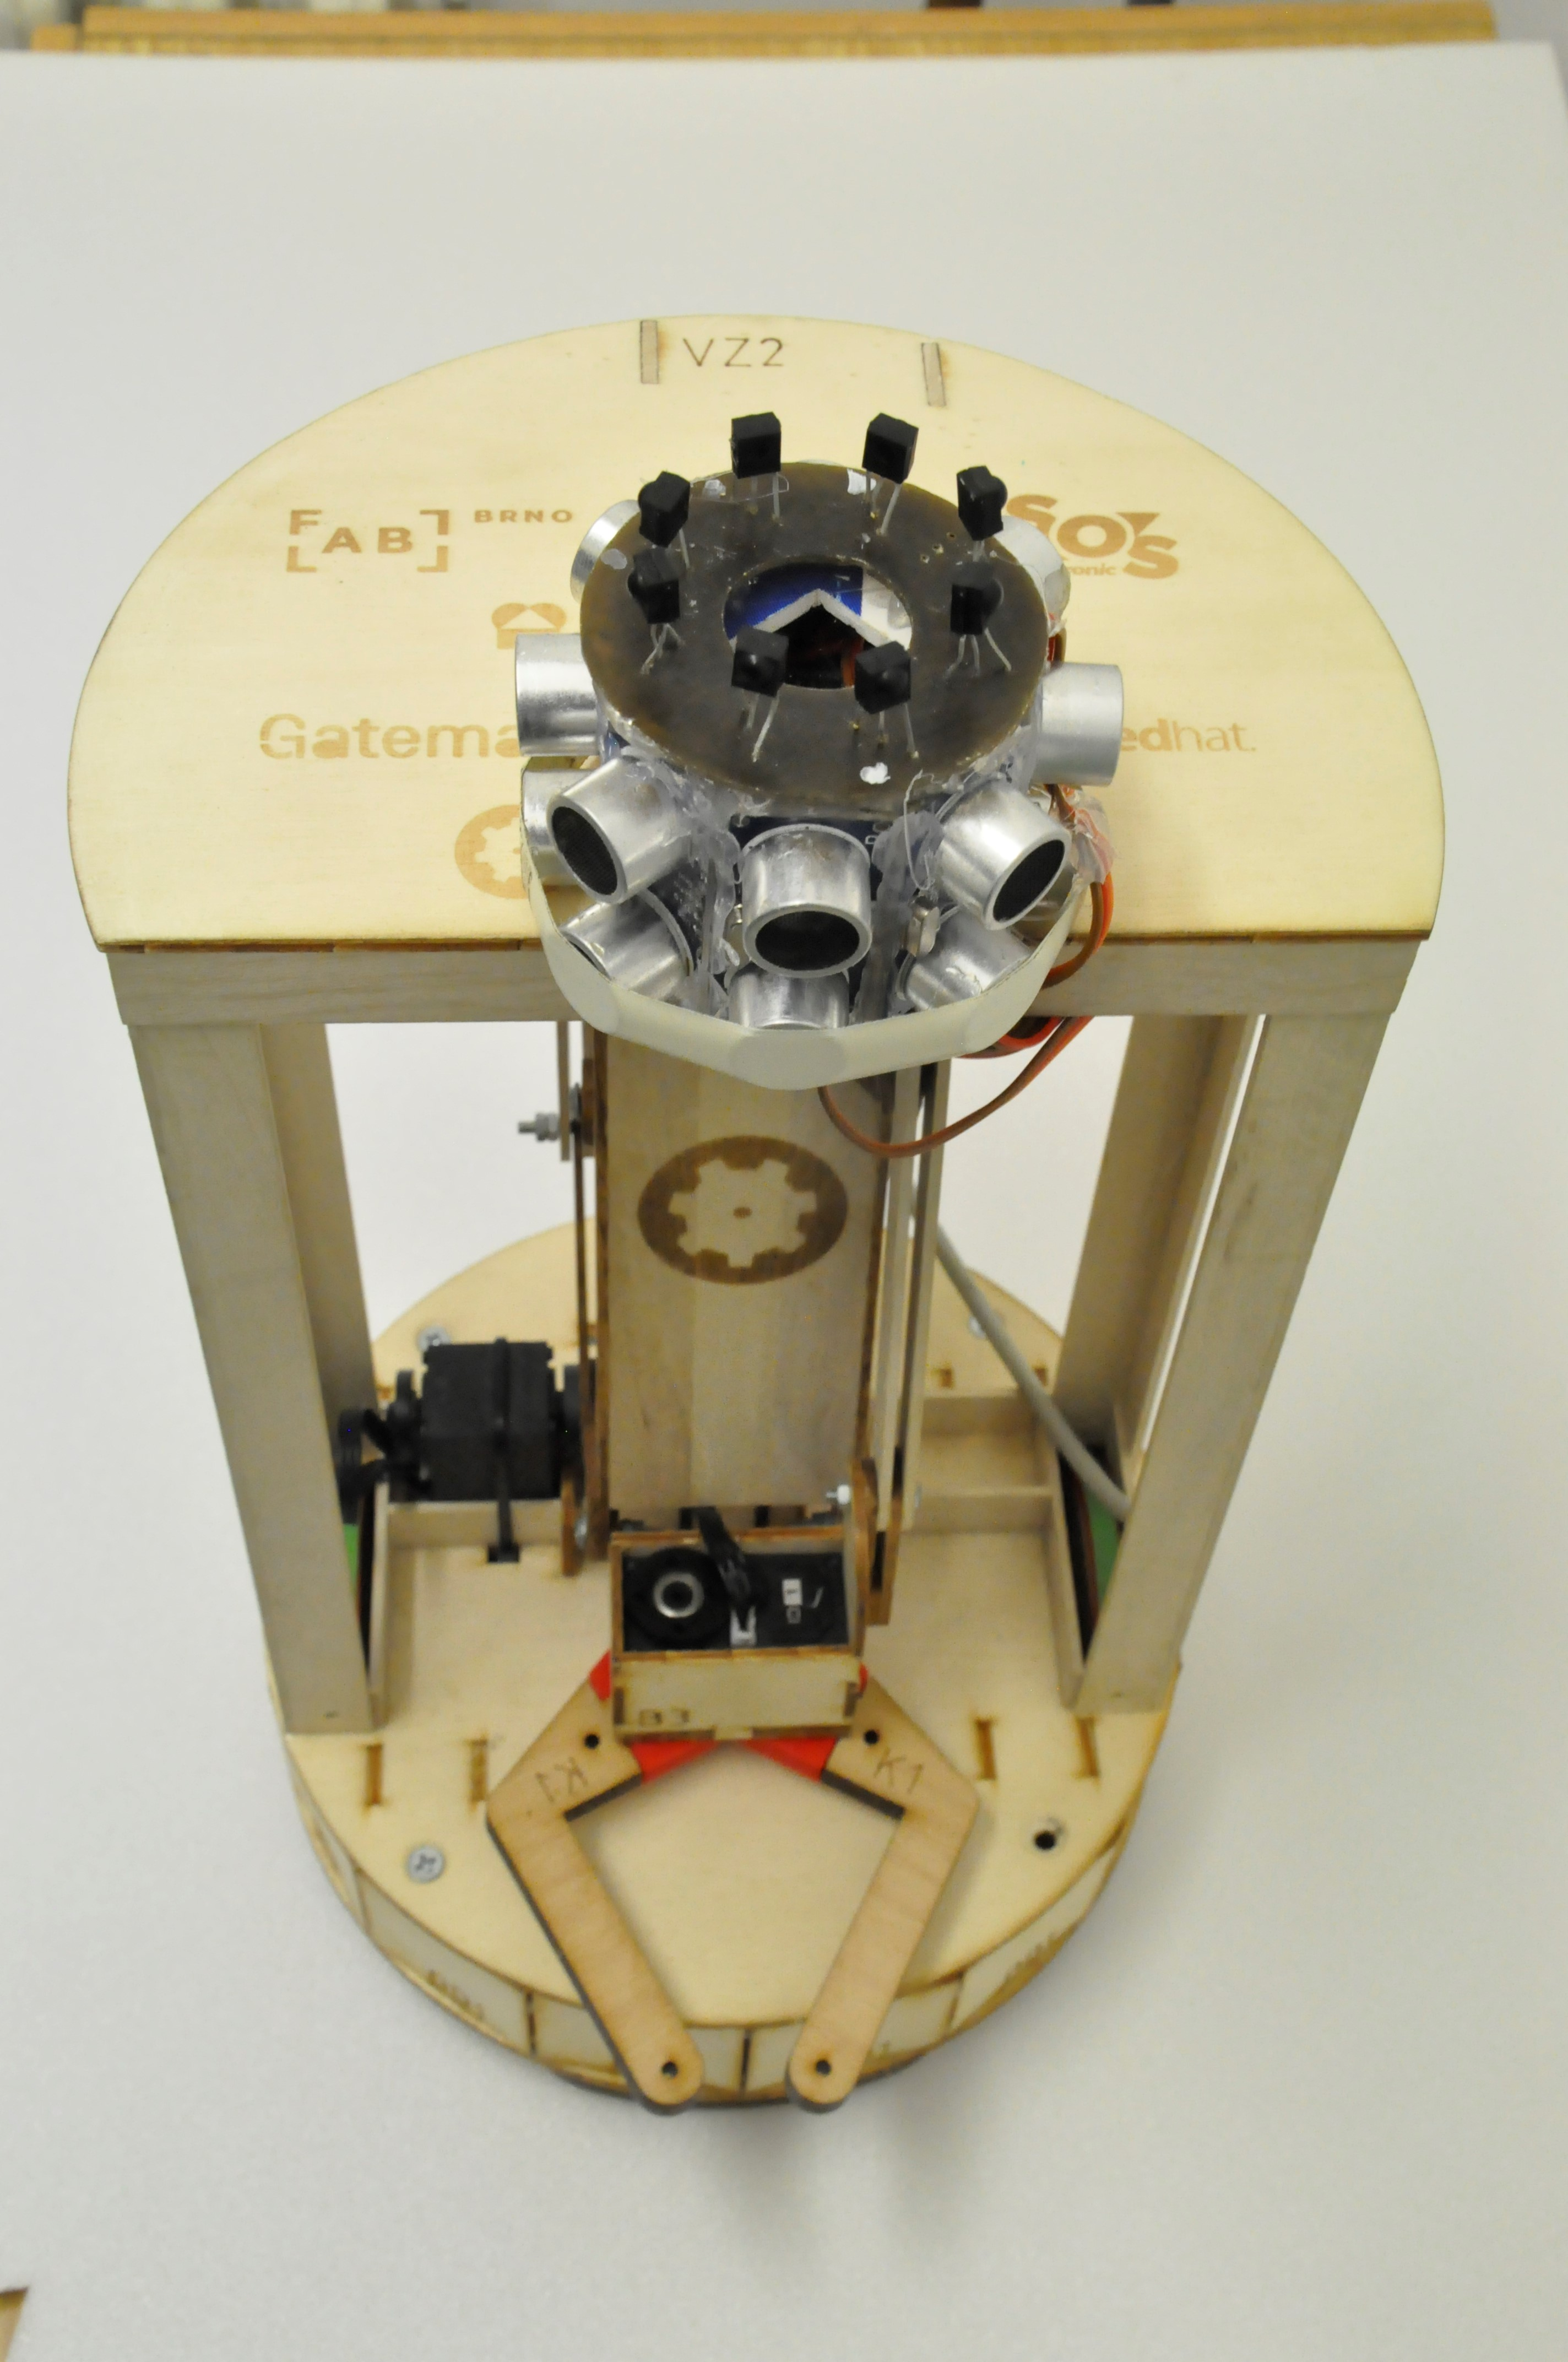
\includegraphics[width=0.85\textwidth]{img/prijimac-3.JPG}
    \caption{Fotografie přijímače Janus omni-ultra na robotovi ukazující redukci počtu vodičů na čtyři díky využití dodatečného procesoru v rámci modulu.}
    \label{fig:prijimac3}
\end{figure}

\begin{figure}[htbp]
    \centering
    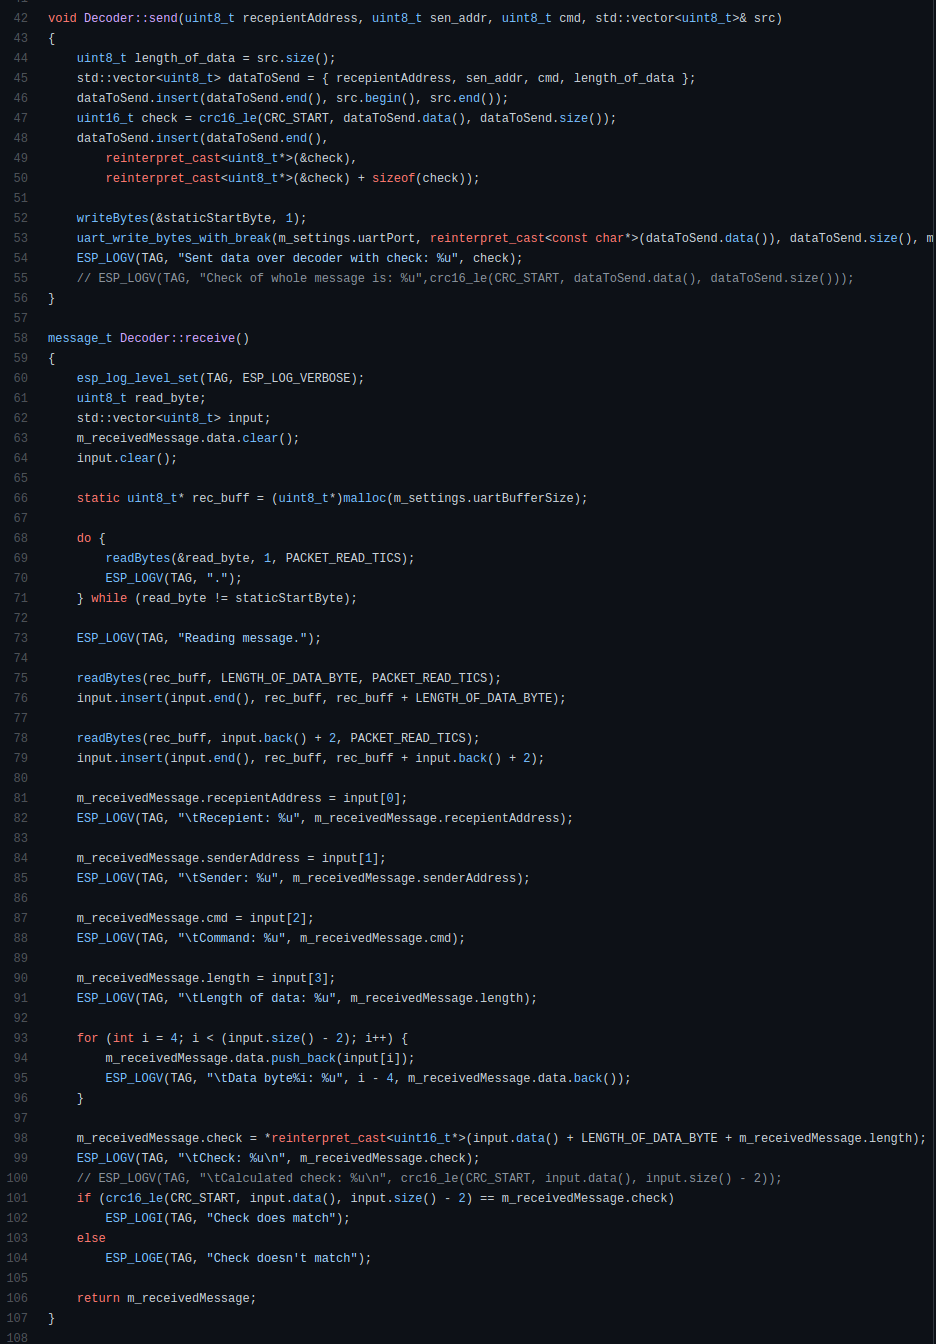
\includegraphics[width=0.85\textwidth]{img/ukazka-kod.png}
    \caption{Ukázka kódu.}
    \label{fig:kod}
\end{figure}

\begin{figure}[htbp]
    \centering
    
\includegraphics[width=0.85\textwidth]{img/participation.jpg}
    \caption{Účastnický list SOČ 2019/2020}
    \label{fig:particip}
\end{figure}

\newpage

\begin{figure}[htbp]
    \centering
    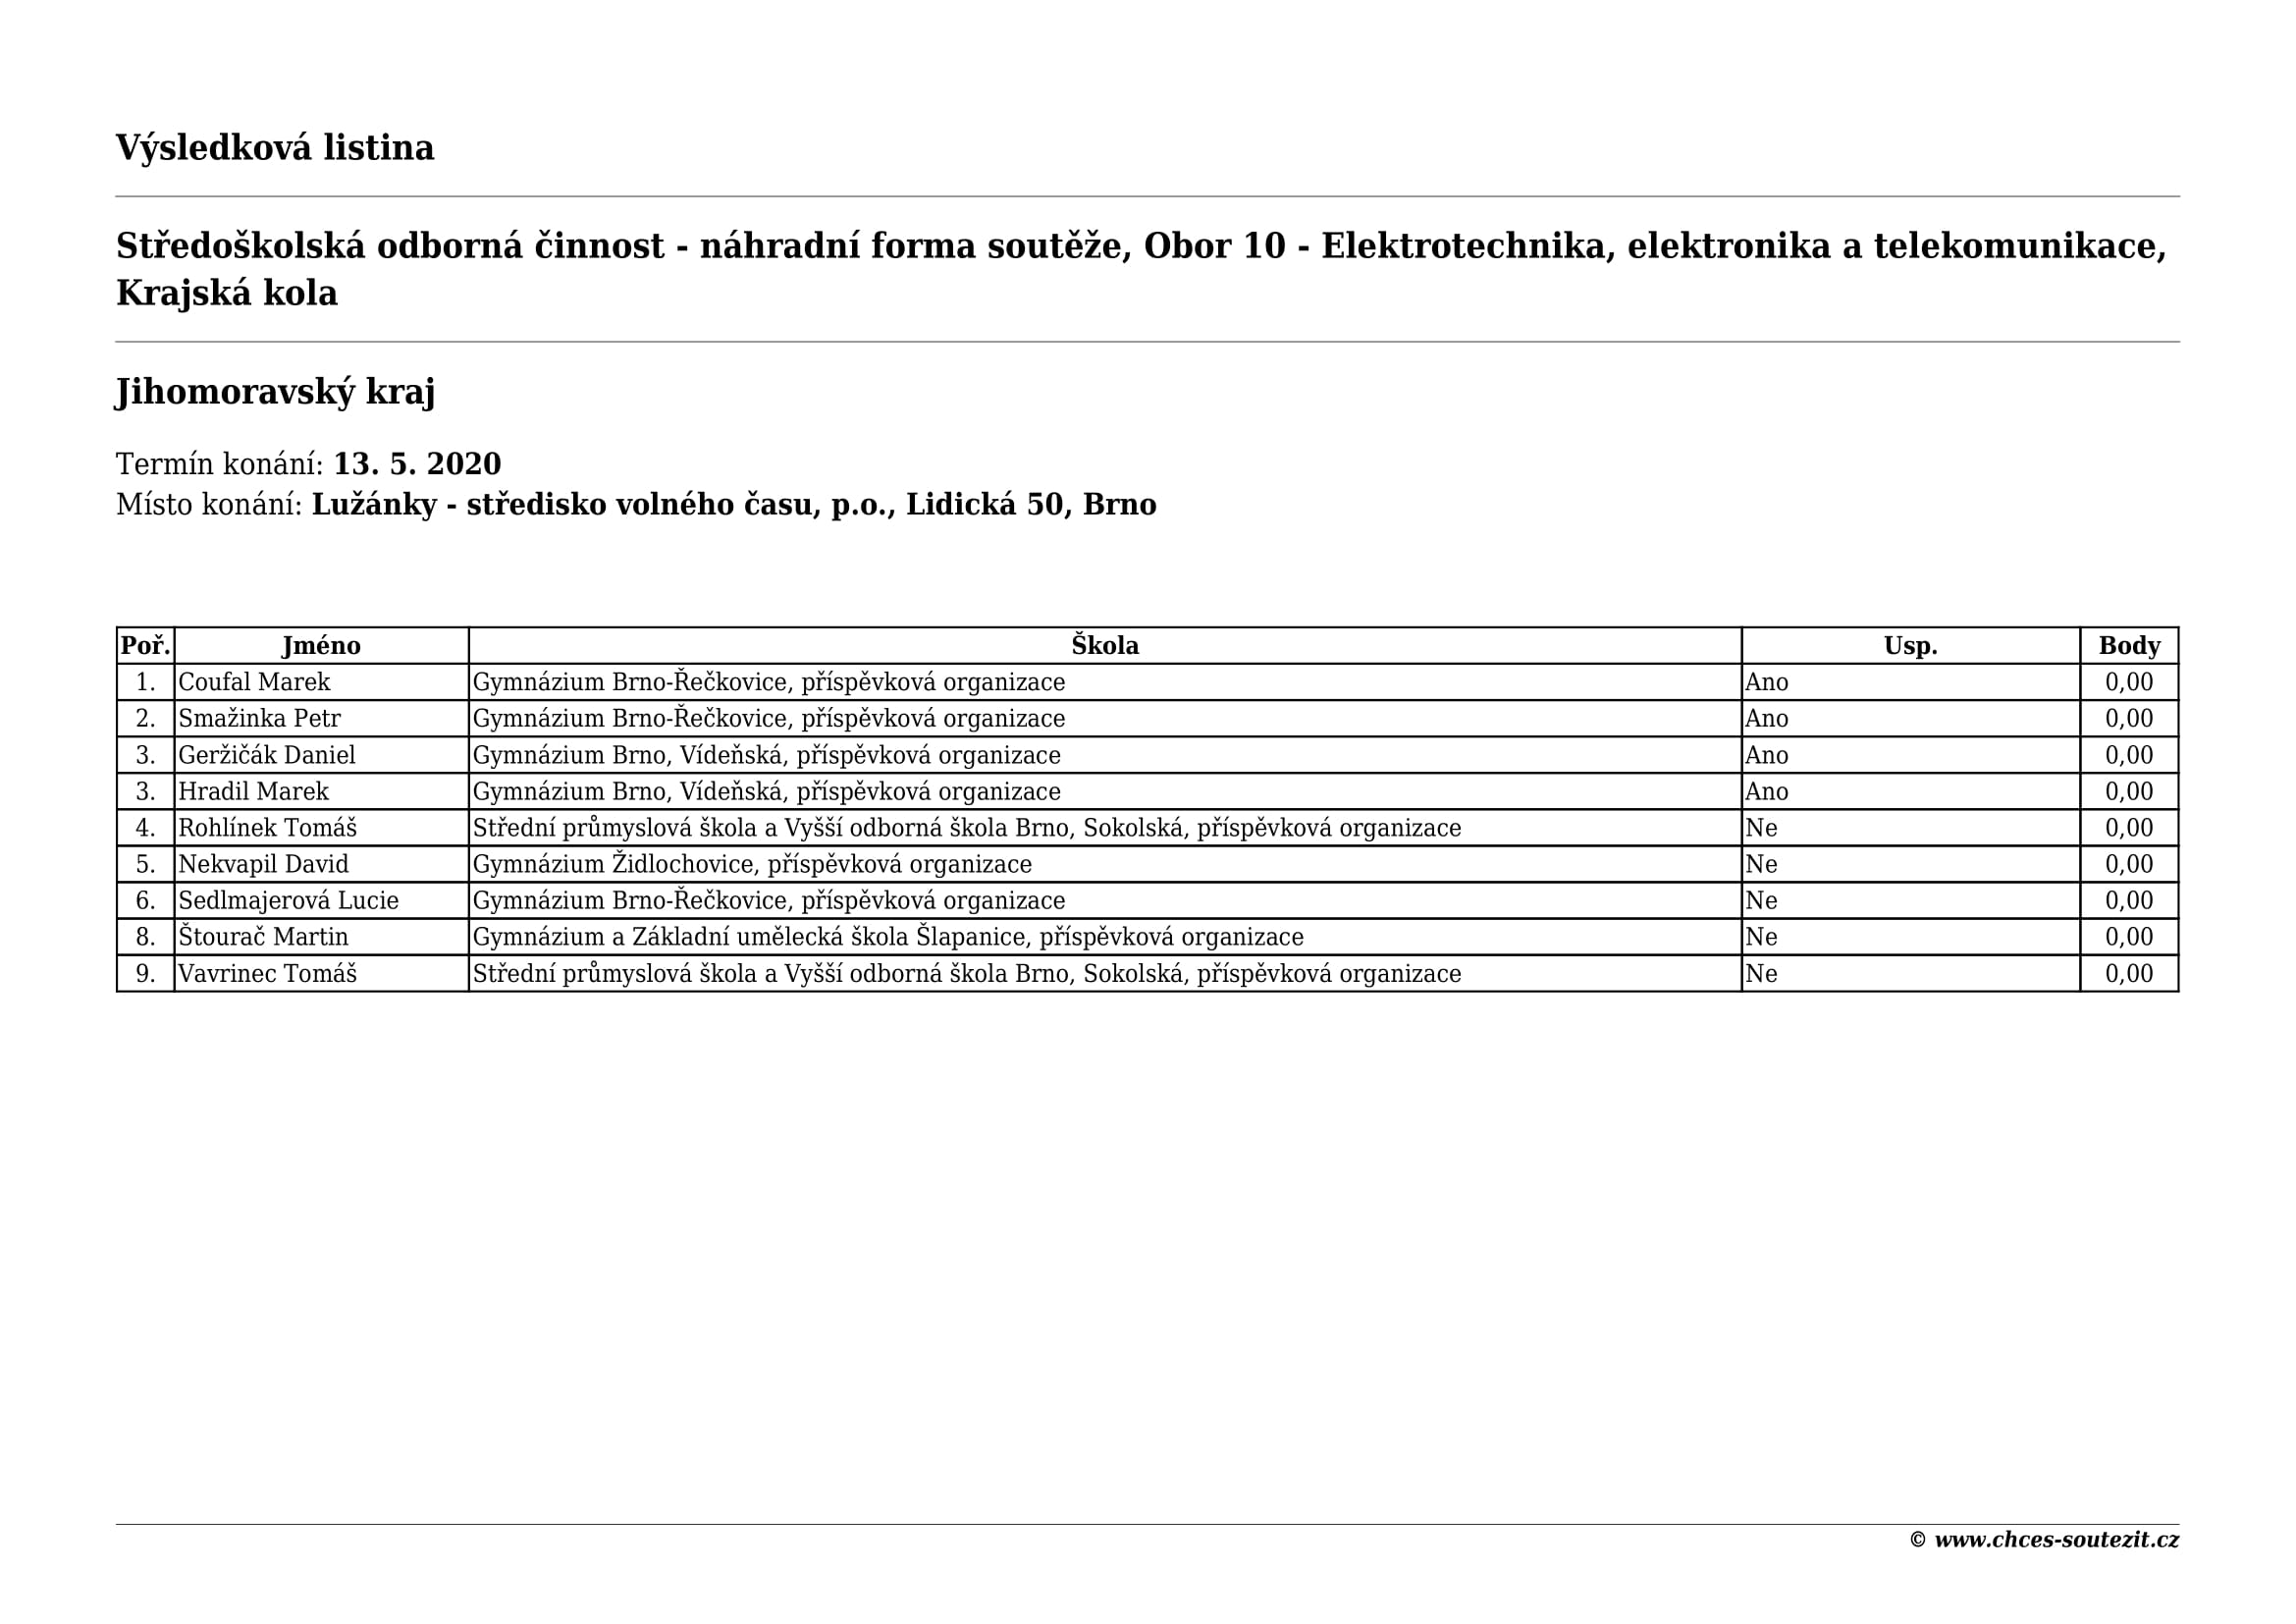
\includegraphics[angle=90,width=0.85\textwidth]{img/results.jpg}
    \caption{Výsledková listina SOČ 2019/2020}
    \label{fig:results}
\end{figure}
